\subsection{Implementation of \texttt{mm\_malloc}}

In order to make the concepts used in \code{mm_malloc} clearer, I will first explain how the dynamic memory allocator is laid out.

\subsubsection{Memory layout of my dynamic memory allocator}

My dynamic memory allocator uses the notion of blocks in the heap that are either allocated or free. To manage free blocks, I use an explicit free list, which will be described later.

Each block is 8-byte (double word) aligned and consists of a header, footer, and payload. Each block is laid out in memory as shown on \autoref{fig:block-layout} below.

\begin{figure}[H]
  \centering
  \hbox{\makebox[\textwidth][c]{
    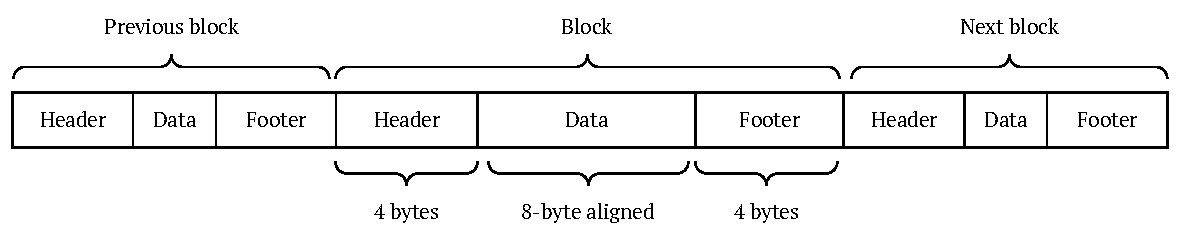
\includegraphics[scale=0.95]{figures/block-layout-example.pdf}
  }}
  \caption{The layout of blocks in memory for my dynamic memory allocator. ``Data'' is used synonymously with ``payload''.}
  \label{fig:block-layout}
\end{figure}

The header consists of the block's size and a flag that indicates if the block is allocated or free. This is all packed into a 32-bit integer. The size of the block is always a multiple of 8, meaning the least significant bit is always 0. Therefore, we can use this single bit to store the allocation flag.

The footer is a duplicate of the header, but it only exists for free blocks.

When we obtain a pointer to a block, the pointer points to the first byte of the payload, not the header.

For allocated blocks, the payload is where the user's data is written to. But for free blocks, because we are using an explicit free list, we use two words (8 bytes) in the payload to store two 4-byte pointers to the next and previous free blocks.

In order to avoid fragmentation, adjacent free blocks are joined every time a block is freed, or if the heap is extended. This means that the blocks in memory are not guaranteed to remain statically laid out --- their sizes can change.

\subsubsection{Components of my \code{mm_malloc} function}

The most important parts of my \code{mm_malloc} implementation (which will all be described in the next sections) are:

\begin{enumerate}
  \item \hyperref[sec:find-fit]{Finding a free block that's large enough}
  \item \hyperref[sec:extend-heap]{Optionally extending the heap}
  \item \hyperref[sec:manipulate-free-list]{Manipulating the free list}
  \item \hyperref[sec:place-block]{Placing the block}
\end{enumerate}

The code examples will use macros and constants for pointer arithmetic and utilities. The definition of these can be seen in \autoref{app:malloc-macros}.

\subsubsection{The explicit free list}
\label{sec:free-list}

It's possible to find a free block on the heap by iterating over all blocks. However, this takes $O(b)$ time (with $b$ being the amount of blocks). Instead, I've implemented an explicit free list, which uses the payload to store pointers to the next and previous free blocks. Using this is a doubly linked list, it's possible to iterate through only the free blocks on the heap, skipping all already-allocated blocks. The structure of free blocks in my implementation is illustrated on \autoref{fig:free-list-structure}.

\begin{figure}[H]
  \centering
  \hbox{\makebox[\textwidth][c]{
    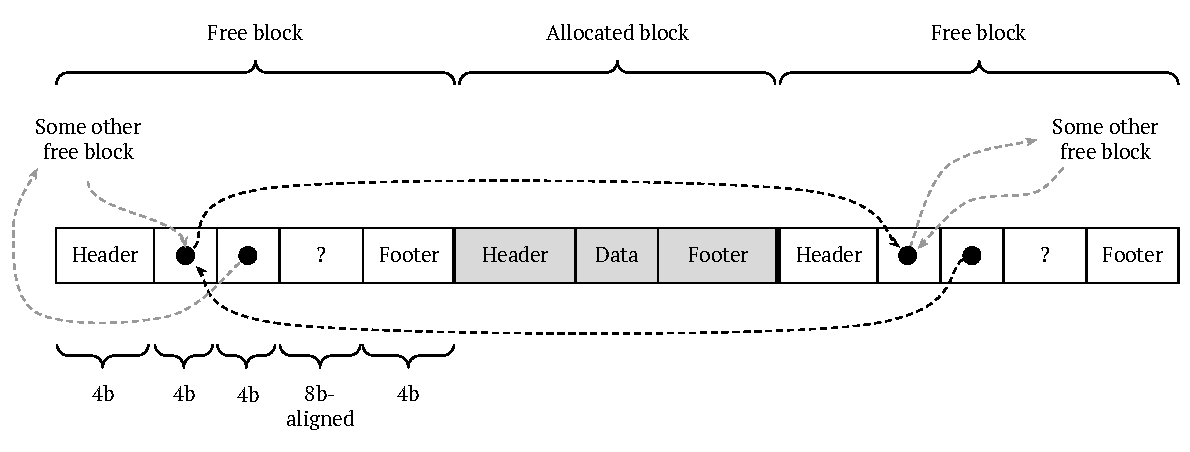
\includegraphics[scale=0.90]{figures/free-list-layout-example.pdf}
  }}
  \caption{An illustration of free blocks in my memory allocator. A block still has a header and footer, but it now also uses the first 8 bytes to store two 4-byte pointers to the next and previous free blocks, respectively. When there is no next or previous free block, the pointer is null. The \code{?} indicates that the rest of the data in a free block is just garbage.}
  \label{fig:free-list-structure}
\end{figure}

With this, it only takes $O(f)$ time (with $f$ being the amount of free blocks) in the worst case to find a free block large enough, if any such block exists.

\subsubsection{Finding a free block that's large enough}
\label{sec:find-fit}

Given the task to find a block of at least size \texttt{size}, it can be done rather straight forward using the explicit free list. Starting at the head of the linked list, we iterate over the entire free list and return a pointer to a free block if that block's size is at least \texttt{size}.

The code for my implementation is as follows:

\bgroup
\small
\begin{minted}[bgcolor=LightGray, linenos]{c}
static void *find_fit(size_t size)
{
    void *block_ptr = free_list;
    while (block_ptr != NULL)
    {
        if (get_size(get_header_ptr(block_ptr)) >= size)
            return block_ptr;

        block_ptr = get_next_free_block_ptr(block_ptr);
    }

    return NULL;
}
\end{minted}
\egroup

As can be seen, I did this using a first-fit search, rather than a best-fit search. This means I use the first block I find rather than the block on the free list where the needed space is as close as the block size as possible. This results in a faster lookup time, but it may cause more fragmentation.

\subsubsection{Optionally extending the heap}
\label{sec:extend-heap}

If no large enough free block can be found, it's necessary to extend the heap to accommodate the allocation request. To do that, the code below is used. An explanation will follow.

Disclaimer: the code for the \code{extend_heap} function has mostly been taken from the course book~\cite[p. 894]{computersystems} but has been modified slightly by me.

\bgroup
\small
\begin{minted}[bgcolor=LightGray, linenos]{c}
/* Increases the size of the heap with the given number of words */
static void *extend_heap(size_t words)
{
    char *bp;
    size_t size;

    /* Allocate an even number of words to maintain alignment */
    size = (words % 2) ? (words + 1) * WSIZE : words * WSIZE;
    if ((long)(bp = mem_sbrk(size)) == -1)
        return NULL;

    /* Initialize free block header/footer and the epilogue header */
    /* Free block header */
    set_val(get_header_ptr(bp), make_header(size, 0));
    /* Free block footer */
    set_val(get_footer_ptr(bp), make_header(size, 0));
    /* New epilogue header */
    set_val(get_header_ptr(get_next_block_ptr(bp)), make_header(0, 1)); 

    add_to_free_list(bp);

    /* Coalesce if the previous block was free */
    return coalesce(bp);
}
\end{minted}
\egroup

Line 8 ensures that the block size is satisfies our alignment.

On line 9, a call to \code{mem_sbrk} is made. This is synonymous to us using the \texttt{void *sbrk(intptr\_t incr)} function in C, which increases the program's data space by \code{incr} bytes \cite{sbrkmanpage}.

I didn't mention this earlier, but the heap is demarcated by two small blocks: the prologue and epilogue. These help the program stop searching at the correct spots. Lines 14-18 show how the empty epilogue block is moved from the current end of the heap to the new end of the heap.

On line 20, the newly allocated block is put onto the explicit free list.

In order to reduce fragmentation when extending the heap and freeing blocks, adjacent free blocks are coalesced into a single free block. This is what happens on line 23.

\subsubsection{Manipulating the free list}
\label{sec:manipulate-free-list}

When a block is allocated, it must be removed from the explicit free list. This works much like a doubly linked list, where addition and removal can be done in constant time. Adding a new free block is done by making it the new head of the list (\autoref{fig:free-list-add}), and removing a block is done by making its predecessor and successor point to each other (\autoref{fig:free-list-remove}).

\begin{figure}[H]
  \centering
  \hbox{\makebox[\textwidth][c]{
    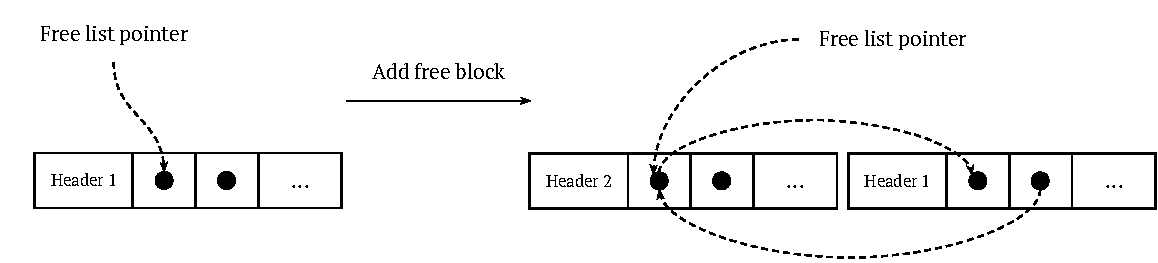
\includegraphics[scale=0.90]{figures/free-list-add-example.pdf}
  }}
  \caption{An illustration showing how to add a free block to the free list.}
  \label{fig:free-list-add}
\end{figure}

\begin{figure}[H]
  \centering
  \hbox{\makebox[\textwidth][c]{
    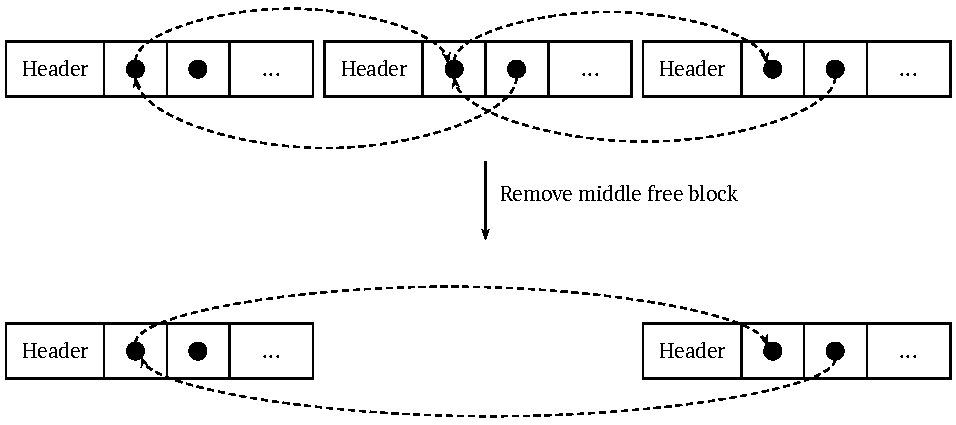
\includegraphics[scale=0.90]{figures/free-list-remove-example.pdf}
  }}
  \caption{An illustration showing how to remove a free block from the free list.}
  \label{fig:free-list-remove}
\end{figure}

The code to obtain that is as follows:

\bgroup
\small
\begin{minted}[bgcolor=LightGray, linenos]{c}
static void add_to_free_list(void *block_ptr)
{
    set_next_free_block_ptr(block_ptr, free_list);
    set_prev_free_block_ptr(free_list, block_ptr);
    set_prev_free_block_ptr(block_ptr, NULL);
    free_list = block_ptr;
}

static void remove_from_free_list(void *block_ptr)
{
    void *prev = get_prev_free_block_ptr(block_ptr);
    void *next = get_next_free_block_ptr(block_ptr);

    if (prev != NULL)
    {
        set_next_free_block_ptr(prev, next);
        set_prev_free_block_ptr(next, prev);
    }
    else
    {
        set_prev_free_block_ptr(next, NULL);
        free_list = next;
    }
}
\end{minted}
\egroup

When removing a block from the free list, there is one extra case to consider: if the block is currently the head of the free list, its successor should become the head of the free list instead. This is what happens on line 21-22.

\subsubsection{Placing the block}
\label{sec:place-block}

Once all the previously described work has been done, the block can be marked as allocated. Recall that it is the least significant bit of the header and footer that store this flag, therefore we simply need to set that bit to 1.

However, we can optimize the allocator with respect to memory utilization. Instead of simply marking the entire block as allocated, we can check if the block has space enough to be split into two blocks: one allocated block that uses just requested amount of space, and one free block with the spare space. This is especially useful because we use first-fit search, meaning the block we find may fit the requested size poorly.

\bgroup
\small
\begin{minted}[bgcolor=LightGray, linenos]{c}
static void place(void *ptr, size_t size)
{
    size_t cur_size = get_size(get_header_ptr(ptr));
    size_t remaining_size = cur_size - size;

    // There is space for another block, so we split
    if (remaining_size >= MIN_BLOCK_SIZE)
    {
        set_val(get_header_ptr(ptr), make_header(size, 1));
        set_val(get_footer_ptr(ptr), make_header(size, 1));

        void *next_block_ptr = get_next_block_ptr(ptr);
        set_val(get_header_ptr(next_block_ptr), make_header(remaining_size, 0));
        set_val(get_footer_ptr(next_block_ptr), make_header(remaining_size, 0));

        // Add the next block to the free list
        add_to_free_list(next_block_ptr);
    }
    // There is not space for another block, so we don't split
    else
    {
        set_val(get_header_ptr(ptr), make_header(cur_size, 1));
        set_val(get_footer_ptr(ptr), make_header(cur_size, 1));
    }
}
\end{minted}
\egroup

The first \texttt{if} block is executed when the found block is large enough to be split into two blocks. The first will be shrunk to the requested size and be marked as allocated. The second will be shrunk to the remaining size and added to the free list.

The \texttt{else} block will be executed if the block is not large enough, and it simply marks the block as allocated.

\subsubsection{The \code{mm_malloc} function}

Putting all the above together, I have implemented \code{mm_malloc} as follows:

\bgroup
\small
\begin{minted}[bgcolor=LightGray, linenos]{c}
void *mm_malloc(size_t size)
{
    // Ignore spurious requests
    if (size == 0)
        return NULL;

    // Adjust block size to include overhead and alignment reqs.
    // Size will always be at least 1 due to the check above
    size_t block_size = calc_block_size(size);

    // Search for a fitting block
    void *block_ptr = find_fit(block_size);

    if (block_ptr == NULL)
    {
        // No fit found. Get more memory.
        size_t extend_size = max(block_size, CHUNKSIZE);
        block_ptr = extend_heap(extend_size / WSIZE);
    }

    // The block is now allocated, so we remove it from the free list
    remove_from_free_list(block_ptr);

    // Write the header and footer to the heap (and split the block if there is
    // space left over)
    place(block_ptr, block_size);

    return block_ptr;
}
\end{minted}
\egroup

The procedure is simply:

\begin{enumerate}
  \item Adjust the requested size to 8 byte-alignment
  \item Find a free block that can fit the size
  \item If no block was found, extend the heap to obtain a free block large enough
  \item Remove the found block from the free list
  \item Mark the block as allocated and return a pointer to it
\end{enumerate}

